\documentclass[handout]{beamer}

% math packages
\usepackage{amssymb}

% theme
\usetheme{Rochester}
\usecolortheme{dove}
\usefonttheme{default}

% make the title BIG
\setbeamerfont{title}{series=\bfseries,size=\Huge, parent=structure}

% remove the side title header
\setbeamertemplate{headline}{}

%gets rid of bottom navigation bars
\setbeamertemplate{footline}{}

%gets rid of navigation symbols
\setbeamertemplate{navigation symbols}{}

% define "head" commands for transitions
\newcommand{\headone}{\centering \bf \Huge}
\newcommand{\headtwo}{\centering \bf \LARGE}
\newcommand{\headthree}{\centering \bf \Large}

% define a "spaceit" command for spacing between paragraphs
\newcommand{\spaceit}{\vspace{10mm}}

% define a "red" command to make text red.
\newcommand{\red}[1]{\textcolor{red}{#1}}
\newcommand{\blue}[1]{\textcolor{blue}{#1}}


% simply the style of the lists
\setbeamertemplate{itemize items}[default]
\setbeamertemplate{enumerate items}[default]

% increase the default spacing between equations
\setlength{\jot}{5pt}

% custom color for "blockcode"
\usepackage{fancyvrb,color}

\DefineVerbatimEnvironment{blockcode}
  {Verbatim}
  {formatcom=\color{blue}}


\begin{document}
\title{Standard Errors in the ML Framework}   
\author{Carlisle Rainey} 
\date{} % remove date 

\frame{\titlepage} 

\frame{
\headtwo
We know how to get our point estimates. \\\vspace{10mm}
}

\frame{
\textbf{Maximum Likelihood Estimation}
\begin{enumerate}
\pause \item Write down a probability model.
\pause \item Find the probability of the data given the parameters--the likelihood function.
\pause \item Take the log and simplify.
\pause \item Maximize.
	\begin{itemize}
	\pause \item Analytically. (Usually difficult or impossible.)
	\pause \item Numerically. (Usually easier.)
	\end{itemize}
\end{enumerate}
}

\frame{
\headtwo
But how do we get standard errors? \\\vspace{10mm}
\pause And what about confidence intervals?
}

\frame[plain]{
Question: Which of these point estimates is more certain?
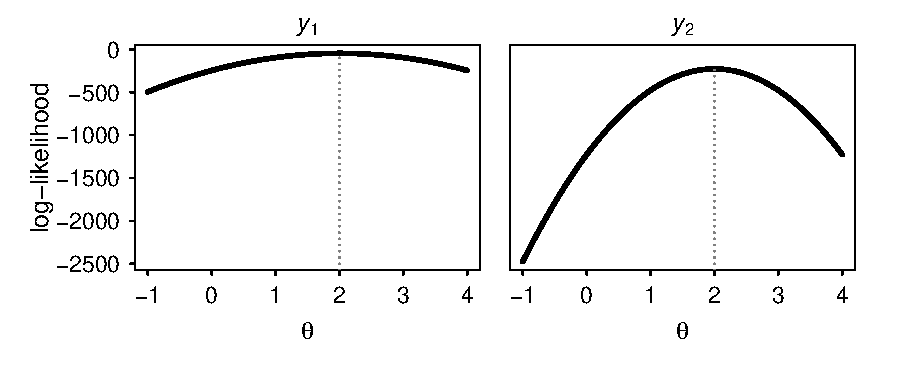
\includegraphics[scale = .7]{figs/curvature.pdf}

\pause Note: These likelihoods are from a normal model with unknown mean. I simulated 100 observations for $y_1$ and 500 observations for $y_2$. (I centered the data so the sample means both occurred exactly at two.)
}

\frame{
\begin{center}
\textbf{\huge{Key Idea}}\\\vspace{10mm}
\pause \Large{We can use the curvature around the maximum likelihood estimate to get a sense of the uncertainty.}
\end{center}
}

\frame{
\begin{center}
\Large{What quantity tells us about the amount of curvature at the MLE?} \\\vspace{10mm}

\red{The second derivative.}\\\vspace{5mm}
\red{second derivative goes down $\rightarrow$ curvature goes up}\\\vspace{3mm}
\red{curvature goes up $\rightarrow$ uncertainty goes down}

\end{center}
}

\frame{
\textbf{Stylized (i.e., $\sigma = 1$) Normal Model Example}
\begin{footnotesize}
\begin{equation*}
\begin{aligned}
\pause \dfrac{\partial \log \mathcal{L}(\mu | y)}{\partial \mu} &= \sum_{i = 1}^n y_i - \mu n\\
\pause \dfrac{\partial^2 \log \mathcal{L}(\mu | y)}{\partial^2 \mu} &=  - n\\
\end{aligned}
\end{equation*}
\end{footnotesize}

\pause Facts:
\begin{enumerate}
\pause \item As $n$ increases, $\frac{\partial^2 \log \mathcal{L}(\mu | y)}{\partial^2 \mu}$ becomes more negative.
\pause \item As $\frac{\partial^2 \log \mathcal{L}(\mu | y)}{\partial^2 \mu}$ gets more negative, the curvature increases.
\pause \item As the curvature increases, the uncertainty decreases.
\end{enumerate}

\begin{center}
\pause Wouldn't it be really nice if we could use $\frac{\partial^2 \log \mathcal{L}(\mu | y)}{\partial^2 \mu}$ to estimate the standard error?
\end{center}
}

\frame{
Single parameter case:
\begin{huge}
\begin{equation*}
var(\hat{\theta}) \approx \left[\left. - \frac{\partial^2 \log \mathcal{L}(\theta| y)}{\partial^2 \theta}\right| _{\theta = \hat{\theta}}\right] ^{-1}
\end{equation*}
\end{huge}

}


\frame{
Continuing the stylized normal example:
\begin{equation*}
\dfrac{\partial^2 \log \mathcal{L}(\mu | y)}{\partial^2 \mu} =  - n
\pause ~{\color{purple}{\Longrightarrow}}~
\left[\left. - \frac{\partial^2 \log \mathcal{L}(\mu | y)}{\partial^2 \mu}\right| _{\mu = \hat{\mu}}\right] ^{-1} 
\pause = \dfrac{1}{n} 
\pause \approx var(\hat{\mu})
\end{equation*}

\begin{equation*}
sd(\hat{\mu}) \approx \sqrt{\dfrac{1}{n}} \pause ~~\red{\leftarrow \text{standard error}}
\end{equation*}

\begin{center}
\pause Does this answer make sense?\\\vspace{5mm}
\pause Hint: What is the standard error of the mean?
\end{center}
}

\frame{
\headtwo
But what about multiple dimensions? \pause What does ``curvature'' mean in multiple dimensions?
}

\frame{
Perspective plots of the log-likelihood function from the beta model.
\begin{center}
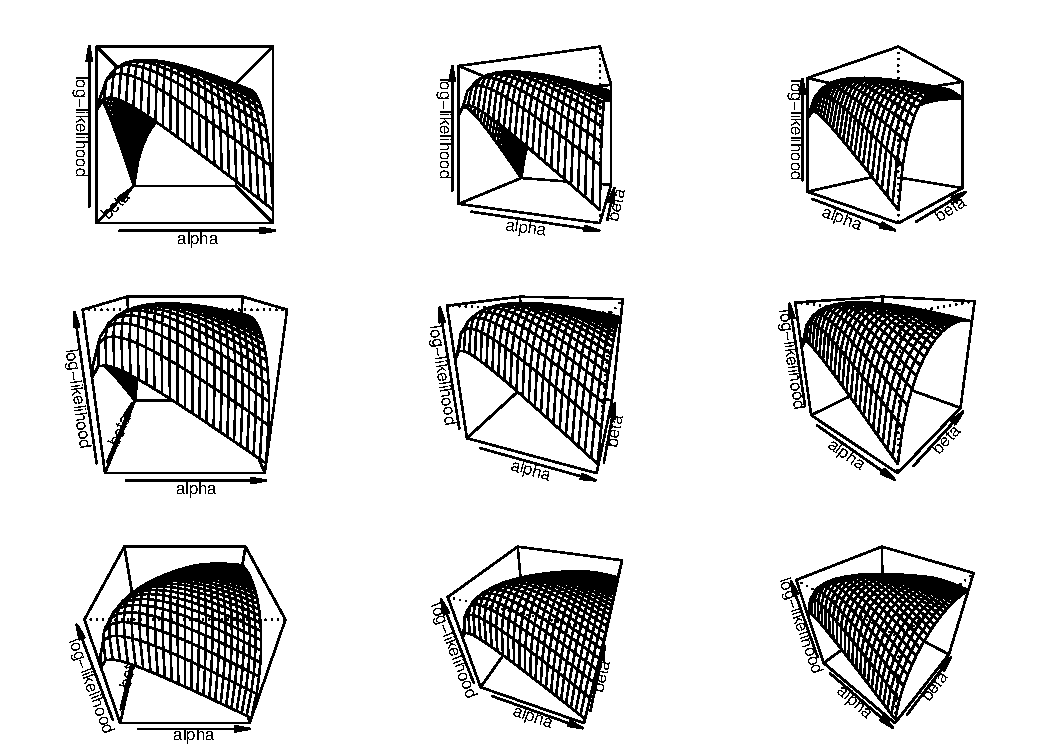
\includegraphics[scale = 0.6]{figs/beta-ll-persp.pdf}
\end{center}
}

\frame{
A contour plot of the log-likelihood function from the beta model.
\begin{center}
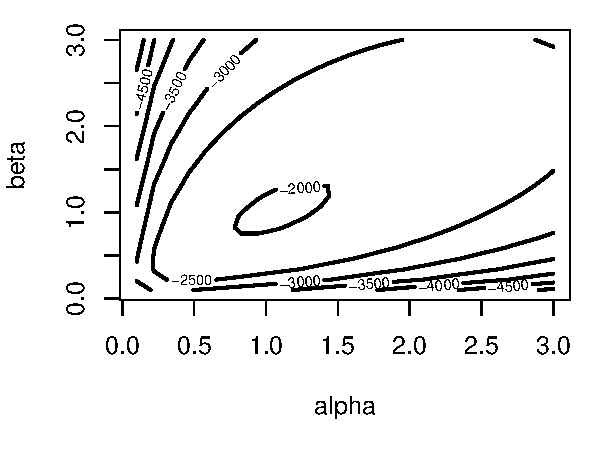
\includegraphics[scale = 1]{figs/beta-ll-contour.pdf}
\end{center}
}

\frame{
\headone
How can we characterize this curvature?
}

\frame{
\headthree
\begin{center}
vertical curvature - the variance of $\hat{\beta}$
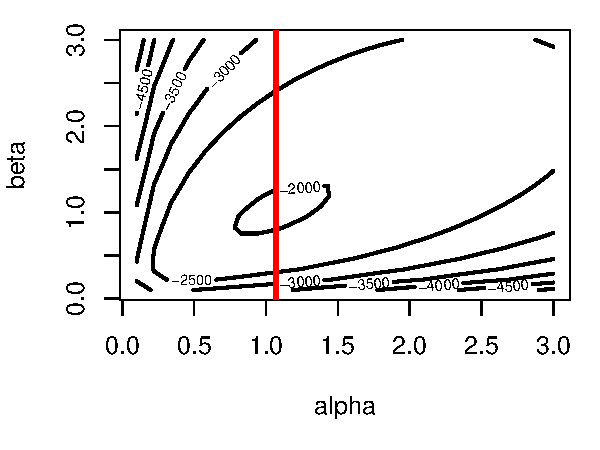
\includegraphics[scale = 1]{figs/beta-ll-contour-vert.pdf}
\end{center}
}

\frame{
\headthree
\begin{center}
horizontal curvature - the variance of $\hat{\alpha}$
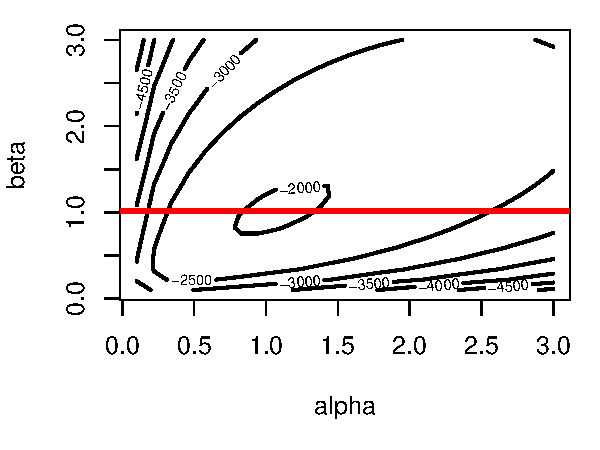
\includegraphics[scale = 1]{figs/beta-ll-contour-horiz.pdf}
\end{center}
}

\frame{
\headthree
\begin{center}
diagonal curvature - the \underline{covariance} of $\hat{\alpha}$ and $\hat{\beta}$
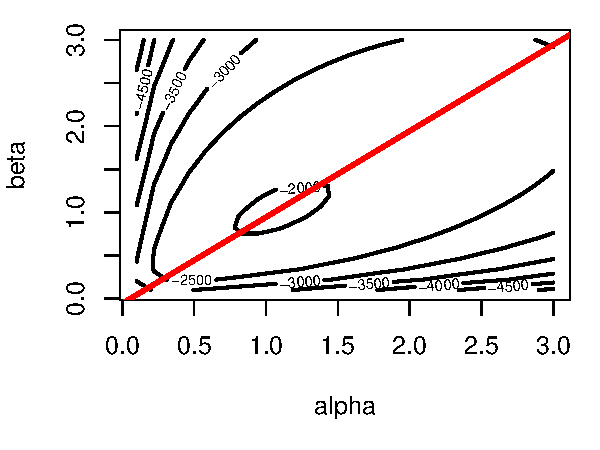
\includegraphics[scale = 1]{figs/beta-ll-contour-diag.pdf}
\end{center}
}

\frame{
\begin{Large}
\begin{equation*}
var(\hat{\theta})= cov(\hat{\theta}) \approx \left. \left[ 
\displaystyle \begin{matrix}
- \frac{\partial^2 \log \mathcal{L}(\theta| y)}{\partial^2 \theta_1} & - \frac{\partial^2 \log \mathcal{L}(\theta| y)}{\partial \theta_1 \partial \theta_2}\\
- \frac{\partial^2 \log \mathcal{L}(\theta| y)}{\partial \theta_2 \partial \theta_1} & - \frac{\partial^2 \log \mathcal{L}(\theta| y)}{\partial^2 \theta_2}\\
\end{matrix}\right]^{-1} \right|_{\theta = \hat{\theta}}
\end{equation*}
\end{Large}
\pause Rather than a single variance, we get a variance \textbf{matrix} (sometimes called the ``covariance matrix'' or the ``variance-covariance matrix'').
}

\frame{
\begin{Large}
\begin{equation*}
var(\hat{\theta})= cov(\hat{\theta}) \approx \left. \left[ 
\displaystyle \begin{matrix}
\red{- \frac{\partial^2 \log \mathcal{L}(\theta| y)}{\partial^2 \theta_1}} & - \frac{\partial^2 \log \mathcal{L}(\theta| y)}{\partial \theta_1 \partial \theta_2}\\
- \frac{\partial^2 \log \mathcal{L}(\theta| y)}{\partial \theta_2 \partial \theta_1} & \red{- \frac{\partial^2 \log \mathcal{L}(\theta| y)}{\partial^2 \theta_2}}\\
\end{matrix}\right]^{-1} \right|_{\theta = \hat{\theta}}
\end{equation*}
\end{Large}
\pause The \red{elements along the diagonal} are the variances for each parameter, so the square root of the diagonal gives you the standard errors. This is exactly what we'd expect.
}

\frame{
\begin{Large}
\begin{equation*}
var(\hat{\theta})= cov(\hat{\theta}) \approx \left. \left[ 
\displaystyle \begin{matrix}
- \frac{\partial^2 \log \mathcal{L}(\theta| y)}{\partial^2 \theta_1} & \blue{- \frac{\partial^2 \log \mathcal{L}(\theta| y)}{\partial \theta_1 \partial \theta_2}}\\
\blue{- \frac{\partial^2 \log \mathcal{L}(\theta| y)}{\partial \theta_2 \partial \theta_1}} & - \frac{\partial^2 \log \mathcal{L}(\theta| y)}{\partial^2 \theta_2}\\
\end{matrix}\right]^{-1} \right|_{\theta = \hat{\theta}}
\end{equation*}
\end{Large}
\pause The \blue{off-diagonal elements} are the covariances--they'll be really important to us later.
}

\frame{
\headone
But what about more than two parameters?\\\vspace{5mm} \pause It's exactly what you'd expect.
}

\frame{
\begin{small}
\begin{equation*}
\begin{aligned}
var(\hat{\theta})= cov(\hat{\theta}) &\approx \left. \left[ 
\displaystyle \begin{matrix}
- \frac{\partial^2 \log \mathcal{L}(\theta| y)}{\partial^2 \theta_1} & - \frac{\partial^2 \log \mathcal{L}(\theta| y)}{\partial \theta_1 \partial \theta_2} & \ldots &- \frac{\partial^2 \log \mathcal{L}(\theta| y)}{\partial \theta_1 \partial \theta_k}\\
- \frac{\partial^2 \log \mathcal{L}(\theta| y)}{\partial \theta_2 \partial \theta_1} & - \frac{\partial^2 \log \mathcal{L}(\theta| y)}{\partial^2 \theta_2} & \ldots & - \frac{\partial^2 \log \mathcal{L}(\theta| y)}{\partial \theta_2 \partial \theta_k}\\
\vdots & \vdots & \ddots & \vdots \\
- \frac{\partial^2 \log \mathcal{L}(\theta| y)}{\partial \theta_k \partial \theta_1}     & - \frac{\partial^2 \log \mathcal{L}(\theta| y)}{\partial \theta_k \partial \theta_2} & \ldots & - \frac{\partial^2 \log \mathcal{L}(\theta| y)}{\partial^2 \theta_k}\\
\end{matrix}\right]^{-1} \right|_{\theta = \hat{\theta}}\\
\pause & \approx \mathcal{I}(\theta)^{-1}|_{\theta = \hat{\theta}}\\
\pause &\approx \mathcal{I}(\hat{\theta})^{-1}
\end{aligned}
\end{equation*}
\end{small}
\pause \textbf{Facts:}
\begin{enumerate}
\pause \item $\mathcal{I}(\hat{\theta})$ is called the [observed] Fisher information [matrix] [at the mle].
\pause \item  $-\mathcal{I}(\hat{\theta}) = \mathcal{H}(\hat{\theta})$ is called the Hessian [matrix].
\pause \item $\sqrt{\text{diag}\left\{\mathcal{I}(\hat{\theta})^{-1}\right\}}$ provides the standard errors of $\hat{\theta}$.
\end{enumerate}
}

\frame{
\headone
What does this mean?
}

\begin{frame}[fragile]
Let's just write a little R function to do the optimization numerically.
\begin{scriptsize}
\pause \begin{blockcode} 
# log-likelihood for beta
ll.fn.beta <- function(theta, y) {
  alpha <- theta[1]  # optim() requires a single parameter vector
  beta <- theta[2]
  ll <- alpha*sum(log(y)) + beta*sum(log(1 - y)) - 
           length(y)*log(beta(alpha, beta))
  return(ll)
}
\end{blockcode}

\pause \begin{blockcode}
# function to estimate beta model
est.beta <- function(y) {
  # optimize log-likelihood
  mle <- optim(par = c(1, 1), fn = ll.fn.beta, y = y,
               control = list(fnscale = -1),
               hessian = TRUE,
               method = "Nelder-Mead") # for >1d problems
  # check convergence
  if (mle$convergence != 0) print("Model did not converge!")
  # pull out and calculate important quantities
  est <- mle$par
  V <- solve(-mle$hessian)
  se <- sqrt(diag(V))
  # put important quantities in list to return
  res <- list(est = est, V = V, se = se)
  return(res)
}
\end{blockcode}
\end{scriptsize}
\end{frame}

\begin{frame}[fragile]
Now let's try a little fake data simulation. This becomes more important now because it let's us test whether our function is working or not.
\pause \begin{blockcode}
# set alpha, beta, and n
alpha <- 2
beta <- 2
n <- 1000
\end{blockcode}

\pause \begin{blockcode}
# simulate the data
set.seed(1234)
y <- rbeta(n, alpha, beta)
\end{blockcode}

\pause \begin{blockcode}
# estimate shape parameters
m1 <- est.beta(y)
\end{blockcode}
\end{frame}

\begin{frame}[fragile]
\begin{blockcode}
> print(m1, digits = 2)
$est
[1] 2.1 2.1

$V
       [,1]   [,2]
[1,] 0.0077 0.0063
[2,] 0.0063 0.0082

$se
[1] 0.088 0.090
\end{blockcode}
\end{frame}

\frame{
\headone
But what about confidence intervals?\\\vspace{5mm}
\headtwo
\pause asymptotics\\\vspace{3mm}
\pause \underline{key} fact: $\hat{\theta} \overset{a}{\sim} N\left[ \theta_{true}, \mathcal{I}(\theta_{true})^{-1}\right]$\\\vspace{5mm} 
}

\frame{
$\hat{\theta} \overset{a}{\sim} N\left[ \theta_{true}, \mathcal{I}(\theta_{true})^{-1}\right]$ implies that he sampling distribution is \textbf{asymptotically normal}. \\\vspace{5mm}

\pause In practice, we'll take this to mean it's \textit{approximately} normal.\\\vspace{5mm}
\begin{align*}
\pause 90\%~\text{C.I.}  &\approx \hat{\theta} \pm 1.64\dfrac{1}{\sqrt{\mathcal{I}(\hat{\theta})}}\\
\pause 95\%~\text{C.I.}  &\approx \hat{\theta} \pm 1.96\dfrac{1}{\sqrt{\mathcal{I}(\hat{\theta})}}
\end{align*}
}

\end{document}
